\documentclass[11pt]{beamer}
\usetheme[pageofpages=of,% String used between the current page and the
                         % total page count.
          bullet=circle,% Use circles instead of squares for bullets.
          titleline=true,% Show a line below the frame title.
          alternativetitlepage=true,% Use the fancy title page.
          ]{Torino}

\usepackage{color}
\usepackage[utf8]{inputenc}
\usepackage[T1]{fontenc}
\usepackage[ngerman,english]{babel}
\usepackage{url}
\usepackage{tangocolors}
\usepackage{tikz}
\usetikzlibrary{arrows,backgrounds,snakes,mindmap}

\setbeamerfont{subtitle}{size=\Large}
\setbeamerfont{author}{size=\large}
\setbeamerfont{institute}{size=\large}
\graphicspath{{img/}}

\author{Daniel Siegel}
\title{On the new threats of social engineering}% exploiting social networks}
\subtitle{exploiting social networks}
\institute{13. August 2009}
\date{}

\begin{document}
\begin{frame}[t,plain]
\titlepage
\end{frame}

\begin{frame}[t]{Inhalt}
  \begin{itemize}
    \item Social Engineering
    \item Soziale Netzwerke
    \item Motivation \& Problemstellung
    \item Ein konkretes Soziales Netzwerk: Twitter
    \item Prototyp
    \item Related Work
  \end{itemize}
\end{frame}

\begin{frame}[t]
\vskip7em
  \begin{center}
    {\Huge Exkurs: Sicherheit in der IT}
  \end{center}
\end{frame}

\begin{frame}[t]
\vspace{-1em}
  \begin{center}
    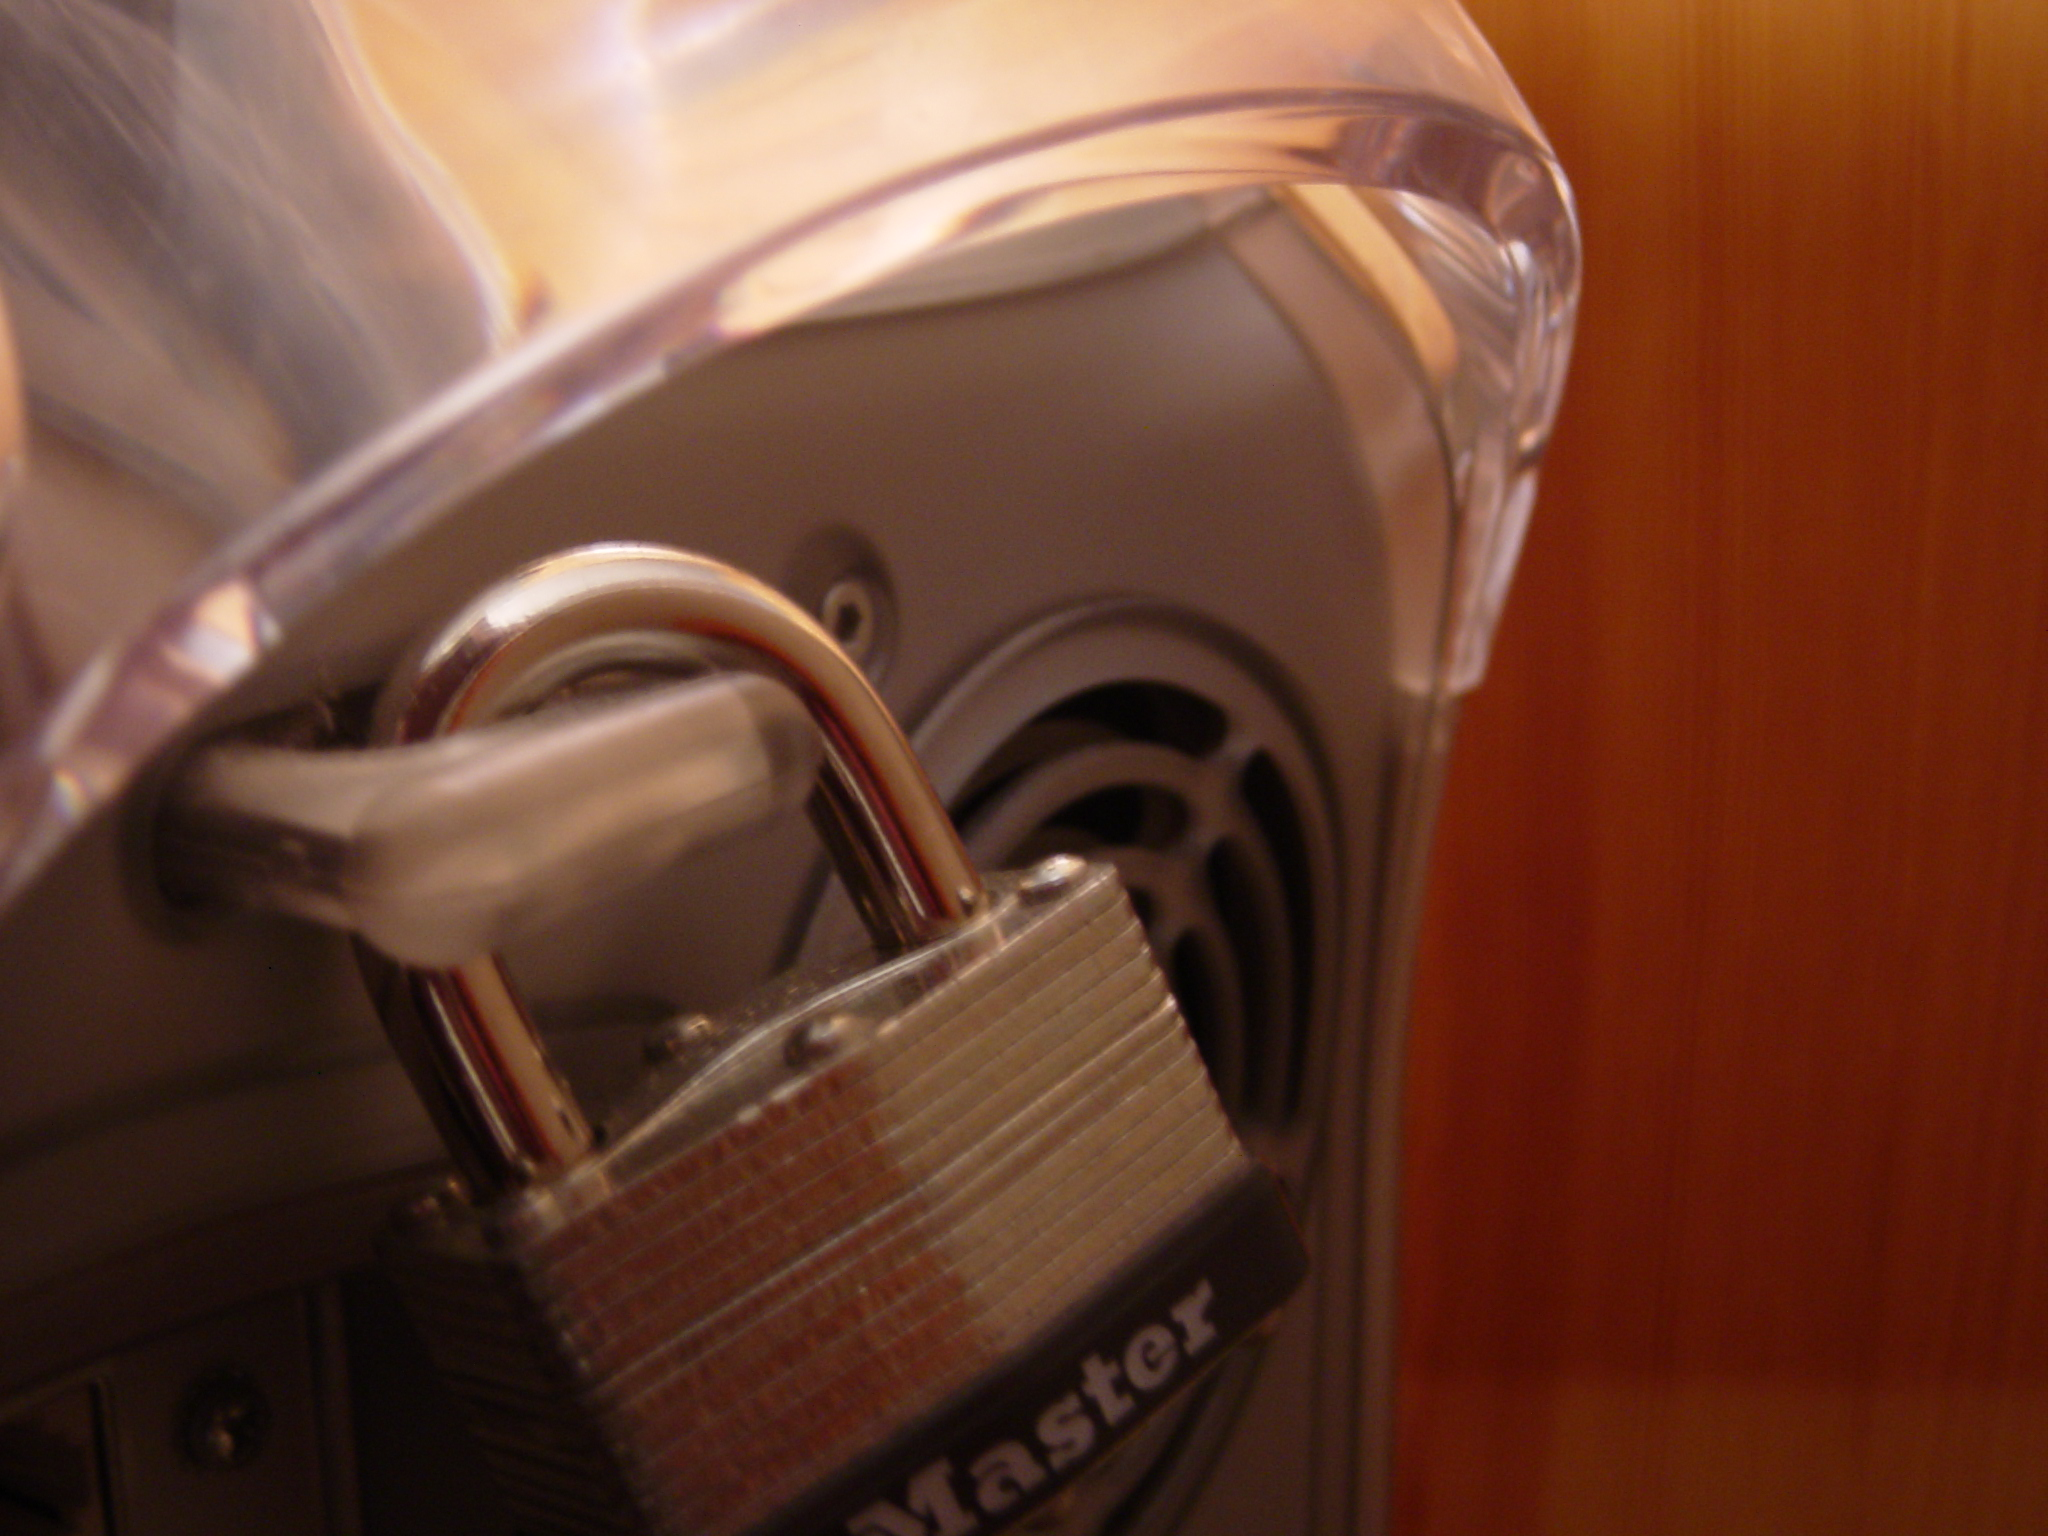
\includegraphics[height=0.95\textheight]{security}
  \end{center}
\end{frame}

\begin{frame}[t]
\vspace{-2em}
  \begin{center}
    
\includegraphics[height=0.95\textheight]{human}
  \end{center}
\end{frame}

\begin{frame}[t]{Definition: Social Engineering}

\vskip3em
\begin{beamercolorbox}[sep=1em]{title page header}
A Term for cracking techniques that rely on weaknesses in wetware rather than
software; the aim is to trick people into revealing passwords or other
information that compromises a target system's security.

\flushright{\scriptsize \glqq{}Social Engineering\grqq{}, The Jargon Dictionary\hskip1em}
\end{beamercolorbox}
\end{frame}

\begin{frame}{Ziele}
  \begin{itemize}
    \item Industriespionage
    \item Identitätsdiebstahl
    \item Spass - Macht
    \item Datendiebstahl
    \item Finanzielle Bereicherung
    \item Soziale Überlegenheit
  \end{itemize}
\end{frame}

\begin{frame}[t]{Verlaufszyklus eines Angriffs}
  \begin{center}
    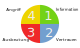
\includegraphics[height=0.75\textheight]{cycle}
  \end{center}
\end{frame}

\begin{frame}{Informationen sammeln}
  \begin{itemize}
    \item Möglichkeiten der Informationsgewinnung
      \begin{itemize}
      \item Firmen-Website
      \item Persönliche Homepage
      \item Dumpster Diving
      \item Phishing
      \item Trojanische Pferde
      \item \dots
      \end{itemize}
    \item Ziel: Informationen $\Rightarrow$ Vertrauen
  \end{itemize}
\end{frame}

\begin{frame}{Vertrauen erarbeiten}
  \begin{itemize}
    \item Informationen
    \item Verantwortung der Handlungen des Opfers entnehmen
    \item Hilfestellung
    \item Beziehung
    \item Stellung
    \item \dots
  \end{itemize}
\end{frame}

\begin{frame}{Ausbeutung, Manipulation \& Angriff}
  \begin{center}
  {\Large
  Stanley Mark Rifkin\\
  vs.\\
  Security Pacific National Bank\\
  Los Angeles
  }
  \end{center}
\end{frame}

\begin{frame}{Ausbeutung, Manipulation \& Angriff}

\begin{beamercolorbox}[sep=1em]{title page header}
\textcolor{skyblue3}{\textit{\glqq{}Hi, this is Mike Hansen in International.\grqq{}}}\\

\glqq{}Whats your office number, please?\grqq{}\\

\textcolor{skyblue3}{\textit{\glqq{}286\grqq{}}}\\

\glqq{}Okay, what's the code?\grqq{}\\

\textcolor{skyblue3}{\textit{\glqq{}4789\grqq{}}}\\

\textcolor{skyblue3}{\textit{\glqq{}I need a transaction of Ten million, two-hundred thousand
dollars.\grqq{}}}\\

\glqq{}Okay, I got that. Now I need the Interoffice settlement number.\grqq{}\\

\textcolor{skyblue3}{\textit{\glqq{}Let me check, I'll call you right
back.\grqq{}}}\\
...

\end{beamercolorbox}
\end{frame}

\begin{frame}{Ausbeutung, Manipulation \& Angriff}
  \begin{center}
  {\Huge \textbf{+ 10.000.000 \$}}
  \end{center}
\end{frame}

\begin{frame}{Angriff - Human Based Attacks}
  \begin{itemize}
    \item Identitätsdiebstahl
    \item Vortäuschen von Ermächtigungen
    \item Technischer Support
    \item Reverse Social Engineering
    \item Shoulder-Surfing
    \item Dumpster-Diving
    \item Persönlicher Auftritt
  \end{itemize}
\end{frame}

\begin{frame}{Angriff - Computer Based Attacks}
  \begin{itemize}
    \item Phishing
    \item Spam
    \item Malware
    \item Suggestion vertrauenswürdiger Quelle
  \end{itemize}
\end{frame}

\begin{frame}[t]{Soziale Netzwerke}
  \begin{center}
    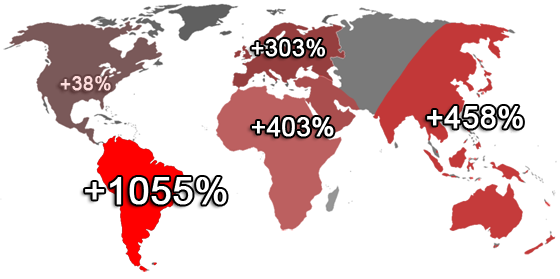
\includegraphics[width=0.75\textwidth]{growth}

    {\tiny
    http://www.techcrunch.com/2008/08/12/facebook-is-not-only-the-worlds-largest-social-network-it-is-also-the-fastest-growing/
    }
  \end{center}
\end{frame}

\begin{frame}[t]{Soziale Netzwerke}
  \begin{center}
    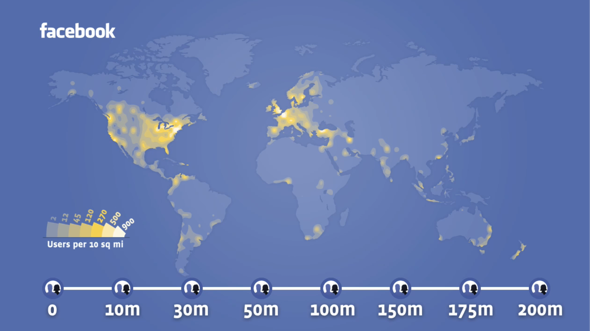
\includegraphics[width=0.75\textwidth]{fbmap}

    {\tiny
    http://venturebeat.com/2009/04/08/trying-to-analyze-facebooks-latest-statistics-more-status-updates-more-content-sharing/
    }
  \end{center}
\end{frame}

\begin{frame}[t]{Verlaufszyklus eines Angriffs}
  \begin{center}
    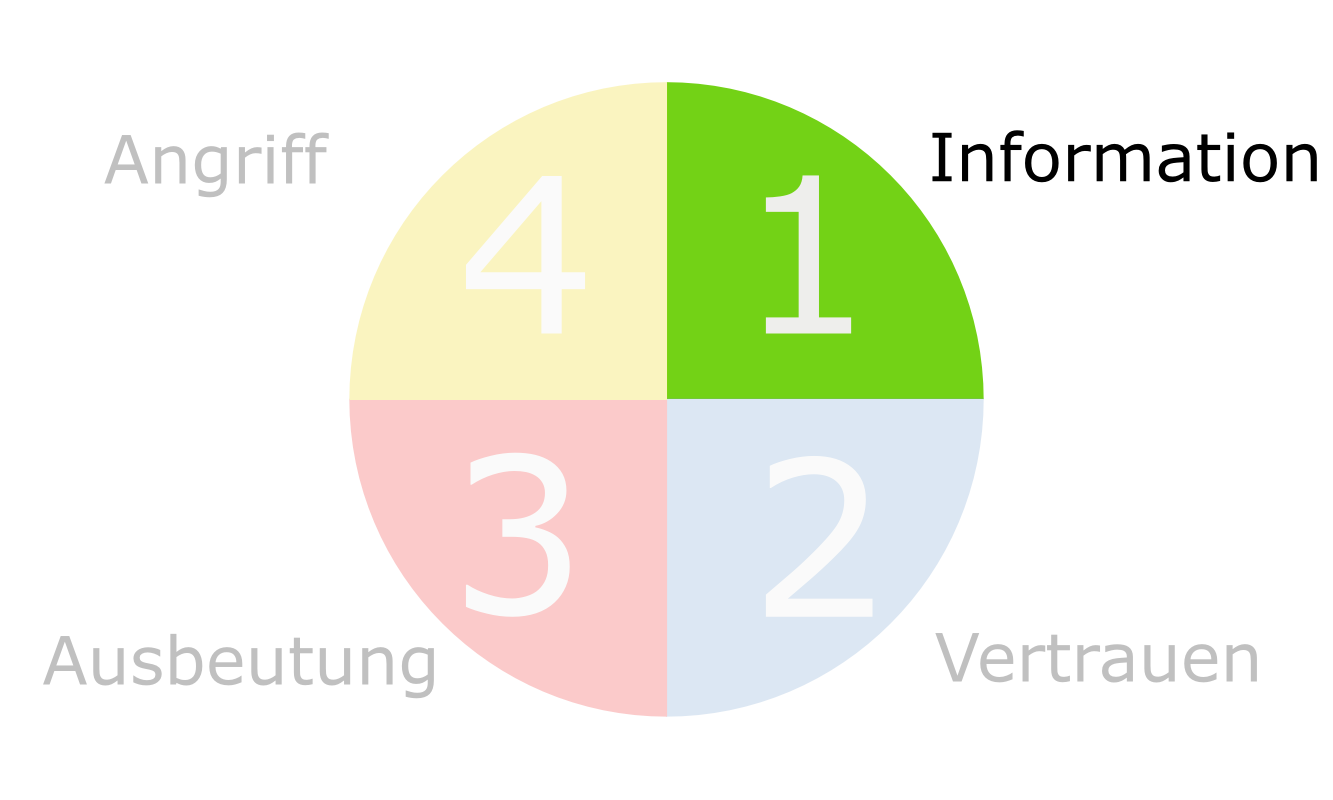
\includegraphics[height=0.75\textheight]{cycle2}
  \end{center}
\end{frame}

\begin{frame}[t]{Problemstellung}

\vskip3em
\begin{beamercolorbox}[sep=1em]{title page header}
Wie können Daten bestimmter
Individuen bzw. Unternehmen über Soziale Plattformen automatisch extrahiert und
so dargestellt werden, dass sie für einen Social Engineering Angriff benutzt
werden können. Zudem sollen Gegenmaßnahmen zu diesen Angriffen erarbeitet
werden.
\end{beamercolorbox}
\end{frame}

\begin{frame}[t]{Ein konkretes Soziales Netzwerk: Twitter}
  \begin{center}
    
\includegraphics[width=0.75\textwidth]{twitter_logo}
  \end{center}
  \begin{itemize}
    \item Soziales Netzwerk \& Microblogging Anbieter
    \item Gegründet 2006
    \item Mehr als $\sim$ 1.500.000 User
    \item Genutzt von Privatpersonen \& Unternehmen
    \item \texttt{http://www.twitter.com/\textit{[username]}}
  \end{itemize}
\end{frame}

\begin{frame}[t]
  \begin{center}
    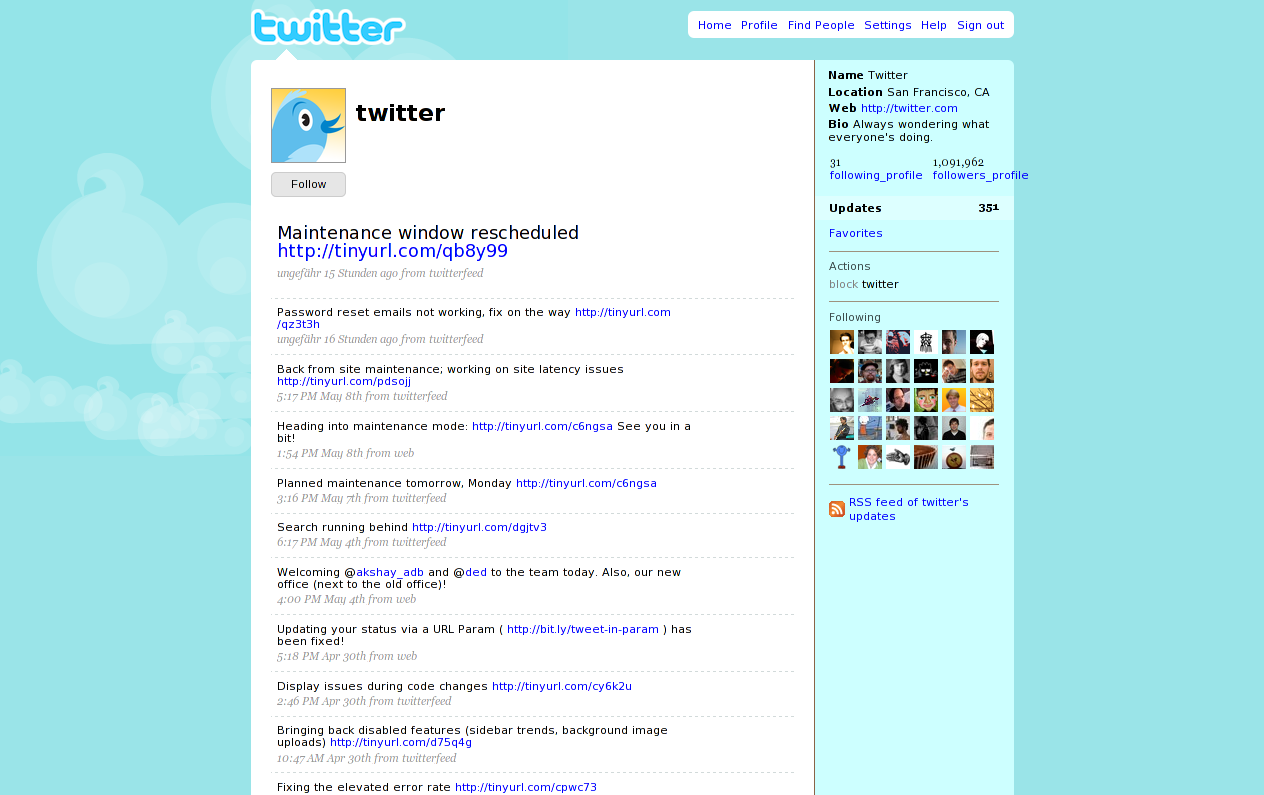
\includegraphics[width=\textwidth]{twitter_home}
  \end{center}
\end{frame}

\begin{frame}[t]{Tweet}
\vskip1em
\begin{beamercolorbox}[sep=1em]{title page header}
\glqq{}@max you should check the weather 
  forecast, see http://tinyurl.com/plmr3m\grqq{}

{\scriptsize \textcolor{aluminium1}{9:34 AM May 28th from web in reply to max}}
\end{beamercolorbox}
\begin{itemize}
  \item 140 Zeichen
  \item @username, \#topic, \dots
  \item Uhrzeit
  \item Benutzte Infrastruktur
  \item reply, new message
  \item Kurz-URL
\end{itemize}
\end{frame}

\begin{frame}[t]
\vspace{-0.85em}
  \begin{center}
    \begin{tikzpicture}[scale=0.65, transform shape,
                         root concept/.append style={concept color=skyblue1},
                         level 1 concept/.append style={concept color=chameleon2},
                         text=white, mindmap]

    \tikzstyle{every annotation}=[fill=skyblue3, font=\sf]

    \node[concept] (Twitter) {Twitter}
      child[concept, grow=160] {node [concept] {Web Interface}}
      child[concept, grow=125] {node [concept] {Twitter API}
      child[concept, grow=left] {node [concept] {User Applications}}}
      child[concept, grow=90] {node [concept] {Facebook}}
      child[concept, grow=55] {node [concept] {IM}}
      child[concept, grow=20] {node [concept] {SMS}}
      %
      child[concept, grow=200] {node [concept] {Web Interface}}
      child[concept, grow=235] {node [concept] {Twitter API}
      child[concept, grow=170] {node [concept] {RSS}}
      child[concept, grow=210] {node [concept] {User Applications}}}
      child[concept, grow=270] {node [concept] {Facebook}}
      child[concept, grow=305] {node [concept] {IM}}
      child[concept, grow=340] {node [concept] {SMS}};

    \node[annotation] at (52.5:7.5) {Twitter Input Methods};
    \node[annotation] at (307.5:7.5) {Twitter Output Methods};

    \draw (2,0) -- (6,0);
    \draw (-2,0) -- (-6,0);

  \end{tikzpicture}
  \end{center}
\end{frame}

\begin{frame}[t]{Twitter API}
\begin{itemize}
  \item http://apiwiki.twitter.com/Twitter-API-Documentation
  \item GET, POST HTML-Methods
  \item GET Anfragen beschränkt auf 100 Requests pro Stunde
  \item json, xml, rss, atom
\end{itemize}
\vskip1em
\begin{beamercolorbox}[sep=1em]{title page header}
\textcolor{plum3}{GET}
http://twitter.com/\textcolor{skyblue3}{users/show}/\textcolor{scarletred2}{barackobama}.\textcolor{aluminium3}{json}
\end{beamercolorbox}
\end{frame}

\begin{frame}[t]{Twitter API (2)}
\begin{beamercolorbox}[sep=1em]{title page header}
{\scriptsize
\begin{tabular}{ll}
created\_at:   &    "Mon Mar 05 22:08:25 +0000 2007"\\
description: &     "The president of the United States of America"\\
favourites\_count: &  0\\
followers\_count:&  1221122\\
friends\_count: &   776706\\
Id:    &       813286\\
location: &        "Chicago, IL"\\
name:   &        "Barack Obama"\\
profile\_image\_url: & "http://s3.amazonaws.com/twitter\_production/ $\hookrightarrow$\\
             &   profile\_images/219314140/obama\_4color\_omark\_normal.jpg"\\
protected:   &   false\\
screen\_name: &   "BarackObama"\\
statuses\_count: &  272\\
time\_zone:  &    "Central Time (US \& Canada)"\\
url:       &   "http://www.barackobama.com"
\end{tabular}
}
\end{beamercolorbox}
\end{frame}

\begin{frame}[t]{Prototyp}
  \begin{center}
    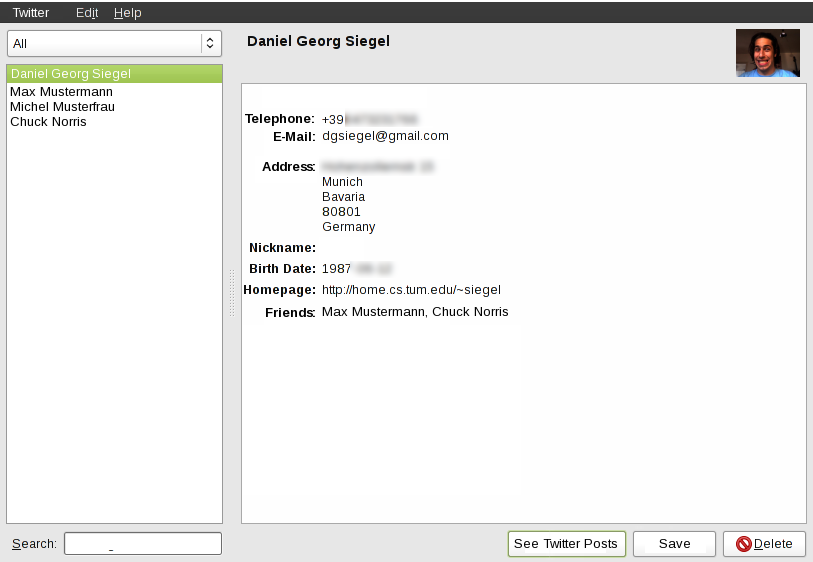
\includegraphics[width=0.85\textwidth]{contacts}
  \end{center}
\end{frame}

\begin{frame}{Szenarien}
  \begin{itemize}
    \item Zeit- und Nutzungsverhalten
    \item Arbeitgeber, Mitarbeiter, Kollegen
    \item Abwesenheit/Urlaube
    \item Telefonnummern, E-Mail Adressen
    \item Geburtstage, Hochzeiten, etc.
    \item ...
  \end{itemize}
\end{frame}

\begin{frame}[t]{Beispiel}
\vskip2em
\begin{beamercolorbox}[sep=1em]{title page header}
\textcolor{plum3}{GET}
http://\textcolor{skyblue3}{search}.twitter.com/\textcolor{skyblue3}{search}.\textcolor{aluminium3}{json}?=\textcolor{scarletred2}{password}
\end{beamercolorbox}
\end{frame}

\begin{frame}[t]{Beispiel (1)}
\vskip2em
\begin{beamercolorbox}[sep=1em]{title page header}
\glqq{}@MattBrewer your nerddinner.com password is "imadork"\grqq{}

\vspace{2em}
{\scriptsize \textcolor{aluminium1}{
22 minutes ago from Tweetie in reply to MattBrewer\\
(http://twitter.com/matt2hews/status/1893008221)
}}
\end{beamercolorbox}
\end{frame}

\begin{frame}[t]{Beispiel (2)}
\vskip2em
\begin{beamercolorbox}[sep=1em]{title page header}
\glqq{}You've been sent a picture message by 447983397493 open it at http://www.vodafone.co.uk/g...  your password is bnh24bfu\grqq{}

\vspace{2em}
{\scriptsize \textcolor{aluminium1}{
40 minutes ago from Ping.fm\\
(http://twitter.com/markiemarkify/statuses/1892911013
}}
\end{beamercolorbox}
\end{frame}

\begin{frame}[t]{Beispiel (3)}
\vskip2em
\begin{beamercolorbox}[sep=1em]{title page header}
\glqq{}@MarkLittlewood Hi Mark, great entry! Google photobucket, login:summerpudding2009 password: summerpudding upload shots with name on\grqq{}

\vspace{2em}
{\scriptsize \textcolor{aluminium1}{
about 1 hour ago from web NickiePhilbin\\
(http://twitter.com/NickiePhilbin/status/1892736072)
}}
\end{beamercolorbox}
\end{frame}

\begin{frame}{Related Work / Social Engineering}
  \begin{itemize}
    \item The Art of Deception
    \begin{itemize}
      \item K. Mitnick, W. Simon
      \item ISBN 076454280X
    \end{itemize}
    \item Social Phishing
    \begin{itemize}
      \item T. Jagatic, N. Johnson, M. Jakobsson, F. Menczer
      \item http://doi.acm.org/10.1145/1290958.1290968
    \end{itemize}
    \item Social Engineering: The “Dark Art”
    \begin{itemize}
      \item T. Thornburgh
      \item http://doi.acm.org/10.1145/1059524.1059554
    \end{itemize}
  \end{itemize}
\end{frame}

\begin{frame}{Related Work / Social Networks}
  \begin{itemize}
    \item Social networks and context-aware spam
    \begin{itemize}
      \item  G. Brown, T. Howe, M. Ihbe, A. Prakash, K. Borders
      \item http://doi.acm.org/10.1145/1460563.1460628
    \end{itemize}
    \item Information revelation and privacy in online social networks
    \begin{itemize}
      \item R. Gross, A. Acquisti, H.  John
      \item http://doi.acm.org/10.1145/1102199.1102214
    \end{itemize}
  \end{itemize}
\end{frame}

\begin{frame}{Related Work / Twitter}
  \begin{itemize}
    \item A few chirps about Twitter
    \begin{itemize}
      \item B. Krishnamurthy , P. Gill, M. Arlitt
      \item http://doi.acm.org/10.1145/1397735.1397741
    \end{itemize}
    \item Why we Twitter
    \begin{itemize}
      \item A. Java, X. Song, T. Finin, B. Tseng
      \item http://doi.acm.org/10.1145/1348549.1348556
    \end{itemize}
  \end{itemize}
\end{frame}

\begin{frame}{Offene Fragen}
  \begin{itemize}
    \item Ersetzen Soziale netzwerke die informationssammlung des Social Engineers?
    \item Analyse weiterer Szenarien, Probleme und Grenzen bei der Informationsgewinnung
    \item Wie sieht ein Generischer Prototyp aus?
  \end{itemize}
\end{frame}

\begin{frame}{Zeitplan}

  \begin{tikzpicture}[thick]
    \filldraw[color=chameleon1] (-3,-1.8) rectangle (-0.2,-1.6)
      node[color=black,pos=0.5,above]{Quellensammlung};

    \filldraw[color=chameleon2] (-0.3,-1.1) rectangle (1.6,-0.9)
          node[color=black,pos=0.5,above]{Related Work};

    \filldraw[color=chameleon3] (0.2,-0.4) rectangle (2.4,-0.2)
          node[color=black,pos=0.5,above]{Analyse};

    \filldraw[color=chameleon1] (2.1,0.3) rectangle (5.7,0.5)
          node[color=black,pos=0.5,above]{Schutzmöglichkeiten};

    \filldraw[color=chameleon2] (3.2,-0.4) rectangle (5.7,-0.2)
          node[color=black,pos=0.5,above]{Evaluation};

    \filldraw[color=skyblue1] (0.5,-1.8) rectangle (1.2,-1.6)
          node[color=black,pos=0.5,above]{API};

    \filldraw[color=skyblue2] (1.7,-1.1) rectangle (4.8,-0.9)
          node[color=black,pos=0.5,above]{Prototyp};

    \filldraw[color=scarletred2] (1.6,-1.8) rectangle (5.0,-1.6)
          node[color=black,pos=0.5,above]{Testen};

    % Axis
    \draw (-3,-2) -- (8,-2);
    % Note that the snaked line is drawn to 11.1 to force
    % TikZ to draw the final tick.
    \draw[snake=ticks,segment length=2.2cm] (-3,-2) -- (8.1,-2);

    % -3.0 April
    % -0.8 Mai
    %  1.4 Juni
    %  3.6 Juli
    %  5.8 August
    %  8.0 September

    \node[below] at (-2,-2) {April};
    \node[below] at (0.2,-2) {Mai};
    \node[below] at (2.4,-2) {Juni};
    \node[below] at (4.7,-2) {Juli};
    \node[below] at (6.9,-2) {August};

    \filldraw[color=chameleon3]  (-3,-3) rectangle (-2.8,-2.8)
          node[color=black,pos=0.5,right]{Wissenschaftliches Arbeiten};
    \filldraw[color=skyblue3]    (-3,-3.4) rectangle (-2.8,-3.2)
          node[color=black,pos=0.5,right]{Entwicklung};
    \filldraw[color=scarletred2] (-3,-3.8) rectangle (-2.8,-3.6)
          node[color=black,pos=0.5,right]{Testen};
  \end{tikzpicture}

\end{frame}

\begin{frame}
  \begin{center}
  {\Huge Fragen?}\\
  {\Large Hinweise?}\\
  {\large Tipps?}\\

\vfill
  \texttt{git clone http://home.cs.tum.edu/siegel/dev/thesis.git}
  \end{center}
\end{frame}

\end{document}
